% !TEX root=week-7-recurrent-networks.tex

\documentclass[10pt]{beamer}
\usepackage{../../../../latex/packages/tslwn-preamble}
\usepackage{../../../../latex/packages/tslwn-slides}
\usepackage{graphicx}
\graphicspath{ {./images/} }

\title{Recurrent networks}
\author{Tim Lawson}

\begin{document}
\maketitle

\begin{frame}
  {Working with sequences\footcite{Karpathy2015}}
  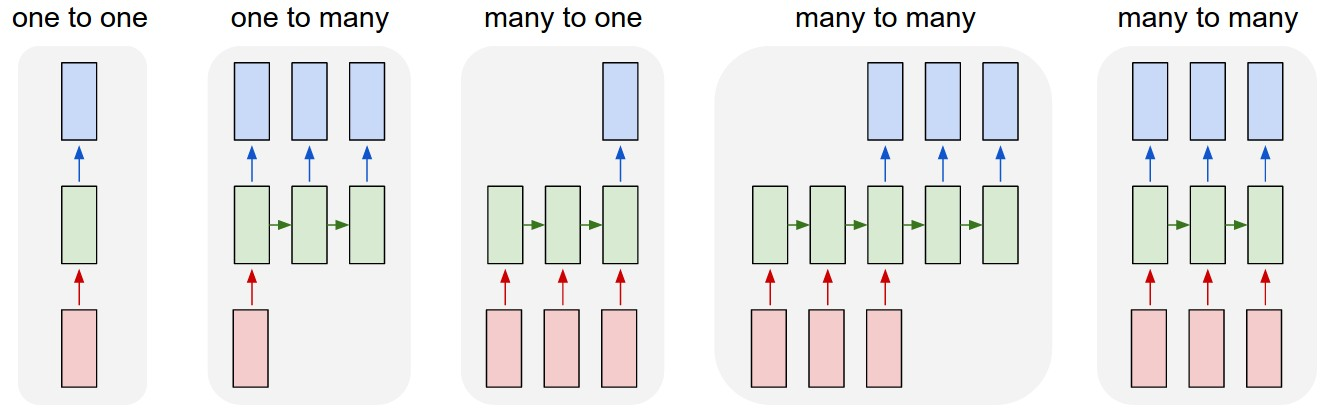
\includegraphics[width=\textwidth]{diags}
  \begin{enumerate}
    \item One-to-one: image classification
    \item One-to-many: image captioning
    \item Many-to-one: sentiment analysis
    \item Many-to-many: machine translation
    \item Many-to-many: video classification
  \end{enumerate}
\end{frame}

\begin{frame}
  {Recurrent vs. feedforward networks\footcite{Mikolov2010}}
  \begin{itemize}
    \item Feedforward networks represent history by \textbf{context}, recurrent
          networks represent history by recurrent network \textbf{connections}.
    \item Feedforward networks have a \textbf{fixed} history length, recurrent
          networks have an \textbf{unlimited} history length.
    \item Feedforward networks compress single words, recurrent networks can
          compress history (\textbf{sequences} of words).
    \item Recurrent networks can form \textbf{short-term memory}.
  \end{itemize}
\end{frame}

\begin{frame}
  {Vanishing gradients}
  \enquote{In theory, the time dependency allows [a recurrent network] in each
    iteration to know about every part of the sequence that came before.
    However, this time dependency typically causes a \textbf{vanishing gradient}
    problem that results in \textbf{long-term} dependencies being
    \textbf{ignored} during training.}\footcite{Madsen2019,Pascanu2013}
  \\~\

  Long short-term memory (\textbf{LSTM})
  networks\footcite{Hochreiter1997,Olah2015} and gated recurrent
  units\footcite{Cho2014} (\textbf{GRUs}) are popular solutions to this
  problem.
\end{frame}

\begin{frame}
  {Bibliography}
  \renewcommand*{\bibfont}{\footnotesize}
  \printbibliography
\end{frame}

\end{document}